%
% File naaclhlt2016.tex
%

\documentclass[11pt,letterpaper]{article}
\usepackage{naaclhlt2016}
\usepackage{times}
\usepackage{latexsym}
\usepackage{float}
\usepackage{graphicx}
\usepackage{hyperref}
\usepackage{listings}
\usepackage[utf8]{inputenc}
\usepackage[T1]{fontenc}
\usepackage{subcaption}
\usepackage{amssymb}
\usepackage{amsmath}
\usepackage{adjustbox}
\usepackage{booktabs}


\naaclfinalcopy % Uncomment this line for the final submission
\def\naaclpaperid{***} %  Enter the naacl Paper ID here

% To expand the titlebox for more authors, uncomment
% below and set accordingly.
% \addtolength\titlebox{.5in}    

\newcommand\BibTeX{B{\sc ib}\TeX}

\lstset{
     literate=%
         {á}{{\'a}}1
         {í}{{\'i}}1
         {é}{{\'e}}1
         {ý}{{\'y}}1
         {ú}{{\'u}}1
         {ó}{{\'o}}1
         {à}{{\`a}}1
         {À}{{\`A}}1
         {ê}{{\'e}}1
         {ù}{{\`{u}}}1
         {è}{{\v{e}}}1
         {š}{{\v{s}}}1 
         {č}{{\v{c}}}1
         {ř}{{\v{r}}}1
         {ž}{{\v{z}}}1
         {ď}{{\v{d}}}1
         {ť}{{\v{t}}}1
         {ň}{{\v{n}}}1                
         {ů}{{\r{u}}}1
         {Á}{{\'A}}1
         {Í}{{\'I}}1
         {É}{{\'E}}1
         {Ý}{{\'Y}}1
         {Ú}{{\'U}}1
         {Ó}{{\'O}}1
         {Ě}{{\v{E}}}1
         {Š}{{\v{S}}}1
         {Č}{{\v{C}}}1
         {Ř}{{\v{R}}}1
         {Ž}{{\v{Z}}}1
         {Ď}{{\v{D}}}1
         {Ť}{{\v{T}}}1
         {Ň}{{\v{N}}}1                
         {Ů}{{\r{U}}}1    
}

\title{Latent Constraints on a Continuous Sentence Space}

% Author information can be set in various styles:
% For several authors from the same institution:
% \author{Author 1 \and ... \and Author n \\
%         Address line \\ ... \\ Address line}
% if the names do not fit well on one line use
%         Author 1 \\ {\bf Author 2} \\ ... \\ {\bf Author n} \\
% For authors from different institutions:
% \author{Author 1 \\ Address line \\  ... \\ Address line
%         \And  ... \And
%         Author n \\ Address line \\ ... \\ Address line}
% To start a seperate ``row'' of authors use \AND, as in
% \author{Author 1 \\ Address line \\  ... \\ Address line
%         \AND
%         Author 2 \\ Address line \\ ... \\ Address line \And
%         Author 3 \\ Address line \\ ... \\ Address line}
% If the title and author information does not fit in the area allocated,
% place \setlength\titlebox{<new height>} right after
% at the top, where <new height> can be something larger than 2.25in

\author{Alejandro Posada \\
	    Mila - Université de Montréal\\
	    2920 Ch. de la Tour\\
        Montreal, QC, Canada H3T 1N8 \\
        {\tt alejandro.posada@umonntreal.ca}
	  \And
	Joseph D. Viviano\\
  	Mila - Université de Montréal\\
  	2920 Ch. de la Tour\\
  	Montreal, QC, Canada H3T 1N8 \\
  {\tt joseph@viviano.ca}}

\date{}

\begin{document}

\maketitle

\begin{abstract}
We propose a method for improving the sentences generated from a continuous latent space, which is learned by a variational autoencoder. We use an actor-critic pair to  post-hoc learn latent constraints that act to increase the \textit{realism} of the generated samples and to generate samples with specific phrase-level properties. We evaluate the model's performance on the Penn Treebank and observe that the constraints do alter the latent space, although the attribute constraint does not work as expected.
\end{abstract}

\section{Introduction}
%What is the motivation behind the project? In general terms, what is the hypothesis that you test and how do you go about doing so?
Deep generative models such as Variational Autoencoders (VAEs) \cite{kingma2013auto,rezende2014stochastic}, Generative Adversarial Networks (GANs) \cite{goodfellow2014generative} and autoregressive models \cite{oord2016pixel} have seen great success in computer vision tasks. However, their application to natural language generation is still limited. The discrete nature of text and the complex semantic structure of text make it difficult for these models to learn the true conditional word distribution. Most previous work is in supervised settings such as image captioning \cite{vinyals2015show} and machine translation \cite{bahdanau2014neural}. Recent attempts at unsupervised text generation have utilized VAEs \cite{bowman2015generating} and GANs \cite{yu2017seqgan,zhang2016generating}. These methods generate smooth, but uncontrollable, latent codes.

The current method for unconditional text generation is of limited practical use: if one wants to sample a sentence without specific attributes, it suffices to pick a random sentence from any corpus. Enforcing constraints at training time requires labeled data and retraining the model for new sets of constraints. An alternative approach is to learn constraints on the latent space after training.

We propose an approach for unsupervised controlled generation of text: our objective is to generate realistic sentences with desired phrase-level attributes. We attempt to generate sentences conditionally with desired phrase attributes (e.g., "adverb phrase", "adjective phrase") from a VAE latent space $z$. We enforce such constraints post-hoc on $z$ using the method from \cite{engel2017latent}. We expect our work to be one of many steps towards achieving fine-grained control of text generation.


\section{Related work}
%Summarize previous work in the area that you have found. I don’t expect you to give a complete and fully up-to-date survey of related work in the area. Instead, aim to cite and discuss at least 3-5 relevant papers, with a focus on how your work differs from theirs.

Several approaches to unsupervised text generation have been proposed. The standard recurrent neural network language model (RNNLM) \cite{mikolov2011extensions} generates each word of a sentence conditioned on the previous word and an evolving hidden state. As a consequence of these prediction scheme, the RNNLM does not capture global features such as syntactic properties and topics. Moreover, RNNLM suffer from exposure bias as they are trained using maixmum likelihood \cite{bowman2015generating}

An alternative approach uses models that capture global features in a continuous latent variable. GANs are a framework for training generative models  where a generator generates samples to fool a discriminator that is trained to discriminate between real and synthetic samples. GANs have been used with moderate success in this task. The main problem with this approach is that since text is discrete, it is not possible to propagate the gradient from the discriminator to the generator. Different solutions for this problem have been proposed: using the Gumbel-softmax distribution \cite{kusner2016gans}, professor forcing \cite{lamb2016professor}, etc. Similarly, Reinforcement Learning has been used by other approaches, including LeakGAN \cite{guo2017long}, SeqGAN \cite{yu2017seqgan}, RankGAN \cite{lin2017adversarial} and MaskGAN \cite{fedus2018maskgan}. An important variant that we incorporate in our work is Conditional GAN (CGAN) \cite{mirza2014conditional}, which is able to produce controlled samples by conditioning both the generator and the discriminator on the labels.

Another method that aims at representing global features in a latent variable is the VAE. This model is a regularized version of the standard autoencoder that imposes a prior distribution on the latent vector $z$. This allows to impose a regular geometry on the $z$ and allows to draw samples via ancestral sampling. Instead of using a deterministic encoder, the VAE uses an inference network to learn the distribution $q_{\theta}(z|x)$ that approximates the posterior $p(z|x)$. The likelihood is parametrized with a generative network $p_{\phi}(x|z)$. The VAE is trained by maximizing the evidence lower bound (ELBO):
\begin{align}
    \mathcal{L}(\theta, \phi, x) = &\mathbb{E}_{q_{\phi}(z|x)} [ \log p_{\theta}(x|z) ] \nonumber \\
    &- \text{KL}(q_{\phi}(z|x) || p_{\theta}(z)) \\ 
    & \leq \log p(x) \nonumber
\end{align}

Works on conditional generation of text are scarce. For example, \cite{rajeswar2017adversarial} present a method to train GANs for natural language and are able to generate sentences conditioned on high-level features such as sentiment and questions. \cite{hu2017toward} proposed a method to control sentiment and tense by focusing on getting disentangled VAE representations in a semi-supervised setting. To the best of our knowledge, no work has tackled the problem of achieving phrase-type control in unsupervised text generation.

\section{Methods}
%Describe the model that you implement, the data set that you use, and any other materials. There should be sufficient details that another researcher is able to more or less replicate your experiment with some effort.
Our framework uses a VAE to generate sentences. We then learn latent constraints to perform conditional generation without re-training the VAE. We impose two constraints: one that enforces similarity to the data distribution and one that helps generate sentences with desired attributes (sentence-level tags)\footnote{Our code is available in \url{github.com/alejandroposada/comp550-project}}.

\subsection{Dataset}
All experiments were done using the Penn Treebank dataset with 42069 parsed sentences in the training set and 7139 parsed sentences for our test set. Preprocessing included tokenization, removal of most punctuation, all numbers converted to the token "N", and infrequently occurring words being replaced with the token "<unk>". The top 9974 words comprised the non-<unk> vocabulary.

\subsection{Sentence-VAE}
We implemented a VAE to generate sentences based on the work from \cite{bowman2015generating}. Both the encoder and the decoder consist of single layer bidirectional gated recurrent units (GRUs) RNNs \cite{cho2014learning}. The units have a hidden state dimension of 256. The words are represented with a learned dictionary of embedding vectors and the size of the embedding layer is 300. The prior is $p(z) = \mathcal{N}(0,I)$. The model was trained for 100 epochs with the Adam optimizer \cite{kingma2014adam} and a learning rate of $10^{-4}$. 

An important issue with this model is that the training tends to quickly bring the KL term of the ELBO to 0 by setting $q(z|x)$ equal to $p(z)$, which implies that no useful information has been encoded in $z$. To prevent this, we used a sigmoid annealing schedule on the KL term and weakened the decoder by using word dropout \cite{iyyer2015deep,kumar2016ask} with a keep rate of 0.75.

%\begin{figure}
%    \centering
%    \includegraphics[width=0.5\textwidth]{fig/vae.png}
%    \caption{Variational autoencoder language model. %Taken from \protect\cite{bowman2015generating}.}
%    \label{fig:vae}
%\end{figure}

\subsection{Latent constraints}
We use the approach from \cite{engel2017latent} to impose attribute and \textit{realism} constraints on the latent space of the VAE. We use an actor-critic pair approach: we train a critic $D$ to discriminate between encodings of the real data $z \sim q(z|x)$ versus samples from the prior $z \sim p(z)$ or transformed prior samples $z' = G(z \sim p(z),y)$. Here, $G$ is the actor and maps vectors $z$ to latent vectors $z'$ conditioned on the desired attributes $y$.

\subsubsection{Realism constraint}
We trained a \textit{realism} critic $D$ to determine whether a given $z$ maps to a sample of high quality. $D(z)$ is trained to enforce similarity to the data distribution by learning to differentiate between samples from the prior $p(z)$ and the marginal posterior $q(z) \triangleq \frac{1}{N} \sum_n q(z|x_n)$. The critic is trained by optimizing the cross-entropy loss with labels $c=0$ for $z \sim p(z)$ and $G(z \sim p(z), y)$, and $c=1$ for $z \sim q(z|x)$:

\begin{align}
    \mathcal{L}_D(z) &= \mathbb{E}_{z \sim q(z|x)}[\mathcal{L}_{c=1}(z)] + \mathbb{E}_{z \sim p(z)}[\mathcal{L}_{c=0}(z)] \nonumber \\ 
    &+ \mathbb{E}_{z \sim G(p(z))}[\mathcal{L}_{c=0}(z)] 
\end{align}
where $\mathcal{L}_{c=0}(z) \triangleq -(1-\log(D(z)))$ and $\mathcal{L}_{c=1}(z) \triangleq -\log(D(z))$. The actor $G$ is trained by optimizing the loss 
\begin{align}
    \mathcal{L}_G(z) = \mathbb{E}_{z \sim p(z)}[\mathcal{L}_{c=1}(G(z)) + \lambda_{\text{dist}} \mathcal{L}_{\text{dist}}(G(z),z)]
\end{align}
where the regularization term $\mathcal{L}_{\text{dist}}(z',z) \triangleq \frac{1}{\bar{\sigma}_z^2} \log(1+(z'-z)^2)$ encourages nearby solutions while allowing exploration (here, $\bar{\sigma}_z$ denotes the scale $\sigma_z(x)$ of the encoder distribution $q(z|x)$ averaged over the training set). We found that $\lambda_{\text{dist}}=0.1$ yields the best results.

\subsubsection{Attribute constraint}
In order to generate sentences with desired attributes, we impose an implicit attribute constraint on the latent space of the VAE. We use a conditional GAN (CGAN) \cite{mirza2014conditional} in the latent space, i.e. we use conditional versions of the actor ($G(z,y)$) and the critic ($D(z,y)$). 

The binary attributes $y$ are the following sentence-level tags (with their number of occurrences in the training set): SBAR (subordinate clause, $n=21612$), PP (prepositional phrase, $n=36143$), ADJP (adjective phrase, $n=11738$), QP (quantifier phrase, $n=7043$), WHNP (wh-noun phrase, $n=8429$) and ADVP (adverb phrase, $n=17321$). These tags were chosen as many are qualitatively different from one another, and they occur with high frequency in the dataset. In order to evaluate the presence of phrase-tags in samples generated from $z$ or $z'$, we built a probabilistic context free grammar ($n=20648$ rules) using the full parses of the Penn Treebank training set (after preprocessing), and used this in the context of a Viterbi chart parser which uses probabilities to return the single most likely parse \cite{klein2003parsing}. Since the runtime of the Viterbi parser is cubic in the length of the input, we truncated parsing of sentences at 15 tokens if the input was longer. We recorded the presence or absence of these phrase tags in the parses of all samples from $z$ or $z'$.

\subsubsection{Training details}
We used the architectures described in \cite{engel2017latent} for $D$ and $G$. The model was trained for 100 epochs with the Adam optimizer \cite{kingma2014adam} with a learning rate of 3e-4. The training procedure is the same as in \cite{gulrajani2017improved}. Additionally, we applied batch normalization \cite{ioffe2015batch} to $G$'s linear layers and spectral normalization \cite{miyato2018spectral} to $D$'s linear layers to stabilize the training. 

\subsection{Dataset}
We trained our models on the Penn Treebank \cite{marcus1993building}, a corpus of syntactically analyzed and annotated English words. We used the standard train/test split in our experiments.
%It is composed of 1,036,580 words and a vocabulary of 10,000 unique words.

\begin{figure*}[t!]
    \centering
    \begin{subfigure}{0.5\textwidth}
        \centering
        \includegraphics[width=0.9\textwidth]{fig/valid_nll.png}
        \caption{Expected log-likelihood (first term of the ELBO).}
    \end{subfigure}%
    ~ 
    \begin{subfigure}{0.5\textwidth}
        \centering
        \includegraphics[width=0.9\textwidth]{fig/kl_valid.png}
        \caption{KL term value of the ELBO and the sigmoid annealing schedule.}
    \end{subfigure}
    \caption{Training curves of the VAE evaluated on the validation set.}
    \label{vae_train}
\end{figure*}

\begin{figure}
    \centering
    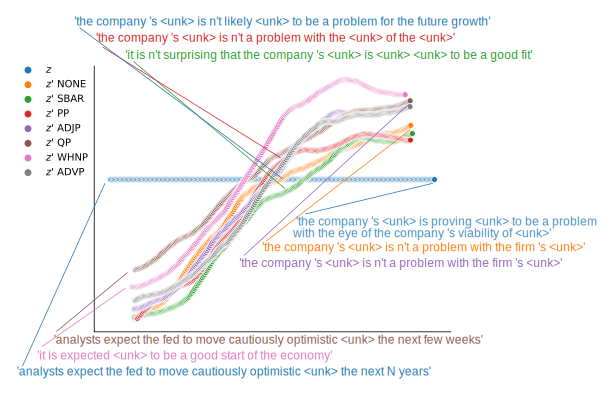
\includegraphics[width=0.5\textwidth]{fig/latent_interp_pretty.png}
    \caption{Low dimensional representation of the latent space interpolation for samples directly from $z$ and samples from $z'$ with each latent attribute constraint.}
    \label{interp}
\end{figure}

\begin{table}[H]
\resizebox{0.49\textwidth}{!}{%
\begin{tabular}{@{}ll@{}}
\toprule
\multicolumn{1}{c}{\textbf{Original}} & \multicolumn{1}{c}{\textbf{Conditioned ADJP}} \\ \midrule
\begin{tabular}[c]{@{}l@{}}

\b{it also would be nice to the company 's <unk>}\\
{\it but it would n't identify the company 's <unk>}\\
{\it but it could n't be reached <unk> for comment}\\
{\it but the company said N it would n't comment on the matter}\\
\b{the company said N it would n't comment on the suit}\\

\end{tabular} & \begin{tabular}[c]{@{}l@{}} 

\b{it also has n't been notified <unk> by the glazer group}\\
{\it it also would n't identify the company 's \\
<unk> pursuit of the company 's <unk>}\\
{\it  but it <unk> n't clear how much money <unk>}\\
{\it  but the company said N it would n't comment on the matter}\\
\b{but the company said N it would n't comment on the suit}\\

\end{tabular} 

\end{tabular}}
\caption{An interpolation through the latent space $z$ and $z'$ conditioned on ADJP.}
\label{interptable}
\end{table}


\section{Results}
%Report the results of your experiment, and any general trends that you see. If the evaluation measure used is not a standard one, be sure to define that as well.
\subsection{Unconstrained language modelling}
Figure \ref{vae_train} shows that the reconstruction term dominates the ELBO and the KL term is not zero. Therefore, the model is able to encode non-trivial information in the latent variable. In Table \ref{interp1} it can be seen that the latent codes contain syntactic information. Not all sentences are grammatical but topic information tends to remain consistent along the path.

\begin{table}[H]
\resizebox{0.45\textwidth}{!}{%
\begin{tabular}{l}
\hline
\textbf{- analysts expect the fed to move cautiously optimistic \textless{}unk\textgreater the next N years} \\
\begin{tabular}[c]{@{}l@{}}- it is expected \textless{}unk\textgreater to be a clear sign that the company's \\ latest purpose isn't regulated, by the end of the 1990s\end{tabular} \\
- the company's \textless{}unk\textgreater isn't likely, to be a problem for the future growth \\
- the company's \textless{}unk\textgreater isn't a problem with the \textless{}unk\textgreater of the \textless{}unk\textgreater{} \\
\textbf{\begin{tabular}[c]{@{}l@{}}- the company's \textless{}unk\textgreater is proving to be a problem with \\ the eye of the company 's viability of \textless{}unk\textgreater{}\end{tabular}} \\ \hline
\textbf{- it also has n't been notified \textless{}unk\textgreater for the past two years} \\
- it also would be nice to the company's \textless{}unk\textgreater{} \\
- but it would n't identify the company's \textless{}unk\textgreater{} \\
- but it would n't elaborate on the matter of the transaction \\
\textbf{- but the company said N it would n't comment on the matter} \\ \hline
\end{tabular}}
\caption{Interpolations between random points in the VAE's latent space.}
\label{interp1}
\end{table}

\subsection{Effect of the attribute constraint}

We conducted chi-square tests to see whether the counts of the phrase-level parse tags were different for samples drawn from $z$ and $z'$ under different attribute constraints. We found a significant difference in the counts when comparing the original $z$ and the $z'$ using no attribute constraints ($\chi^2=13.49, p=0.019$), but no significant differences between the tag-counts of samples drawn from $z'$ with different attribute constraints ($\chi^2=0.85-3.07, p=0.69-0.97$). We conclude that the realism constraint driving most changes in the sentences. This result can be visualized by projecting a linear interpolation between samples taken from two points in $z$ to a two-dimensional space, and superimposing that same trajectory through $z'$ when conditioned on each, or no, attribute constraints (Figure \ref{interp}, Table \ref{interptable}). It is clear that each attribute constraint produces a different trajectory through $z'$, however, each is not always different enough from the others to produce a different set of tokens, and other differences are minor. Trajectory taken by all $z'$ samples are very different from that taken by $z$, and produces different sentences that are still reasonable. We believe the attributes used as a latent constraint did not contain enough useful syntactic information for the actor to successfully learn the sentence structure associated with each tag. However, there were a few exceptions (Table \ref{exception}).

\begin{table}[H]
\resizebox{0.49\textwidth}{!}{%
\begin{tabular}{@{}ll@{}}
\toprule
\multicolumn{1}{c}{\textbf{Original}} & \multicolumn{1}{c}{\textbf{Conditioned}} \\ \midrule
\begin{tabular}[c]{@{}l@{}}columbia owes its creditors as part of its\\  bankruptcy-law reorganization plan \\ because it has been forced \textless{}unk\textgreater to file \\ for bankruptcy protection\end{tabular} & \begin{tabular}[c]{@{}l@{}}{[}\textbf{ADJP}{]} columbia owes the thrift 's\\  \textbf{largest} client claimed N it  would\\  have to pay off the thrift 's \textless{}unk\textgreater{}\end{tabular} \\ \midrule
\begin{tabular}[c]{@{}l@{}}but the japanese government may threaten \\ to manipulate the markets unless it 's too \\ easy to tell whether it 's a good interest\end{tabular} & \begin{tabular}[c]{@{}l@{}}{[}\textbf{PP}{]} but the japanese government 's\\ is proving \textless{}unk\textgreater to be a good bet \textbf{on}\\ the market\end{tabular}
\end{tabular}}
\caption{Conditional generation of sentences. The conditional tag is shown in brackets.}
\label{exception}
\end{table}

\begin{table*}[h]
\centering
\begin{tabular}{@{}ccccccccc@{}}
\multicolumn{9}{c}{\textbf{Train}} \\  \midrule
$z$    & $z'$ mean       & $z'$ NONE & $z'$ SBAR & $z'$ PP & $z'$ ADJP & $z'$ QP & $z'$ WHNP & $z'$ ADVP \\
242.44 & \textbf{165.75} & 169.96    & 171.19    & 176.49  & 158.82    & 161.21  & 157.48    & 166.08    \\
\multicolumn{9}{c}{\textbf{Test}} \\  \midrule
$z$    & $z'$ mean       & $z'$ NONE & $z'$ SBAR & $z'$ PP & $z'$ ADJP & $z'$ QP & $z'$ WHNP & $z'$ ADVP \\
214.71 & \textbf{151.31} & 156.33    & 154.92    & 158.63  & 145.52    & 150.14  & 142.16    & 152.20   
\end{tabular}
\caption{Perplexity scores for samples taken from $z$ and $z'$ using unigram frequencies estimated from both the training and test sets (lower is better).}
\label{perplexity}
\end{table*}


\subsection{Effect of the realism constraint}

The benefit of the realism constraint becomes apparent when evaluating perplexity from the unigram occurrences of the samples drawn from $z$ and $z'$. Expected frequencies were estimated from the training and validation set separately. Table \ref{perplexity} shows a large decrease in perplexity for all samples drawn from $z'$ relative to those drawn from $z$ regardless of the attribute constraint. However we should cautiously interpret this result because perplexity is not a good measure of characteristics such as grammaticality and fluency. 

%\begin{figure*}[t]
%    \centering
%    \begin{subfigure}{0.5\textwidth}
%        \centering
%        \includegraphics[width=0.9\textwidth]{fig/g_loss.%png}
%        \caption{Actor $G$ loss.}
%    \end{subfigure}%
%    ~ 
%    \begin{subfigure}{0.5\textwidth}
%        \centering
%        \includegraphics[width=0.9\textwidth]{fig/d_loss.%png}
%        \caption{Critic $D$ loss.}
%    \end{subfigure}
%    \caption{Training curves of actor-critic pair used to %impose latent constraints on the VAE.}
%\end{figure*}

\section{Discussion and conclusion}
We conclude that adding constraints on the latent space of a sentence VAE model is useful for generating more realistic sentences, as determined qualitatively and by the decrease in perplexity, but believe the major benefit we observe is due to the realism constraint, and more work will be necessary to successfully generate sentences with desired phrase-level attributes. We believe that conditioning on more information from the parse trees, including possibly conditioning on the entire parse tree, will be benefitial, as this will give the model more information regarding which to draw a sample from $z'$.
%What conclusions can be drawn from your experiments? Was your initial hypothesis verified? What are the limitations of your work, and how could it be extended?

\section*{Contributions}
JDV and AP designed the experiments, implemented the VAE, generated results, participated in debugging, refactoring, hyperparameter tuning, and wrote the report. JDV implemented all parsing and corpus generation, conducted follow up analysis, and visualizations. AP implemented the actor critic model and contributed the literature review.

%Briefly describe each member’s contribution. All project members are expected to contribute to the project. While each member may perform different tasks, you should strive for an equal distribution of work. In particular, all members of the project should participate in the design of the project, be involved in writing, and be involved in the ximplementation in some way.


\bibliography{naaclhlt2016.bib}
\bibliographystyle{naaclhlt2016}


\end{document}